\section{Creating View}
\hrulefill

\begin{itemize}
    \item Create a view to display the details of managers and their associated teams
\end{itemize}
\begin{lstlisting}[caption={ ManagerTeamView },label={lst:V-1}]
    CREATE VIEW ManagerTeamView AS
    SELECT m.Manager_Name, t.Team_Name, t.Team_Country
    FROM Manager m
    JOIN Team t ON m.Manager_ID = t.Manager_ID;
\end{lstlisting}
\begin{figure}[H]
    \centering
    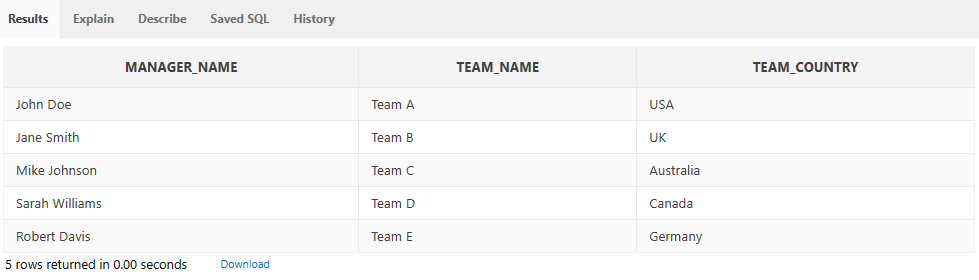
\includegraphics[width=1\textwidth]{images/dml/views/v1.png}
    \caption{Result of ManagerTeamView}
\end{figure}
%%%
\begin{itemize}
    \item Create a view to show the average salary of content creators
\end{itemize}

\begin{lstlisting}[caption={ AvgSalaryView },label={lst:V-2}]
    CREATE VIEW AverageSalaryView AS
    ELECT AVG(ContentCreator_Salary) AS Average_Salary
    ROM ContentCreator;
\end{lstlisting}
\begin{figure}[H]
    \centering
    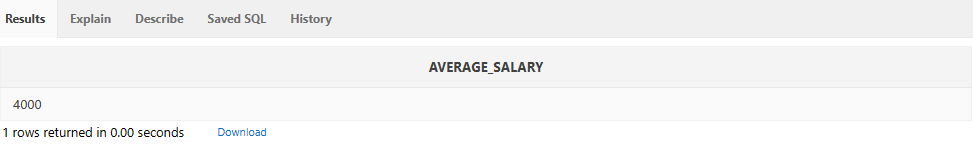
\includegraphics[width=1\textwidth]{images/dml/views/v2.png}
    \caption{Result of AverageSalaryView}
\end{figure}
%%%
\begin{itemize}
    \item Create a view to list the players and their corresponding teams
\end{itemize}
\begin{lstlisting}[caption={ PlayerTeamView },label={lst:V-3}]
    CREATE VIEW PlayerTeamView AS
    JOIN Team t ON pt.Team_ID = t.Team_ID;
    SELECT p.Player_Name, t.Team_Name
    FROM Player p
    JOIN Player_Team pt ON p.Player_ID = pt.Player_ID
\end{lstlisting}
\begin{figure}[H]
    \centering
    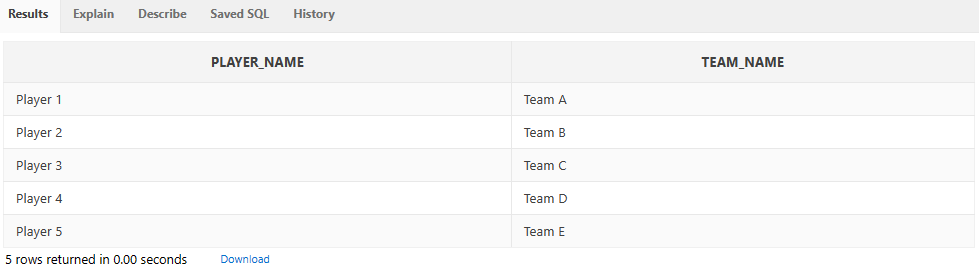
\includegraphics[width=1\textwidth]{images/dml/views/v3.png}
    \caption{Result of PlayerTeamView}
\end{figure}
